\chapter{Background}\label{ch:term}

\section{Introduction}

Image processing is a method to perform some operations on an image, in order to get an enhanced image or to extract some useful information from it. It is a type of signal processing in which input is an image and output may be image or characteristics/features associated with that image~\cite{dip}. In this work we deal with a broad spectrum of image processing techniques.

Morphological image analysis is the subsection of Digital Image Processing that we are most interested in. Binary images may contain numerous imperfections. In particular, the binary regions produced by simple thresholding are distorted by noise and texture. Morphological image processing pursues the goals of removing these imperfections by accounting for the form and structure of the image. These techniques can be extended to greyscale images.

Morphological image processing is a collection of non-linear operations related to the shape or morphology of features in an image. morphological operations rely only on the relative ordering of pixel values, not on their numerical values, and therefore are especially suited to the processing of binary images. Morphological operations can also be applied to greyscale images such that their light transfer functions are unknown and therefore their absolute pixel values are of no or minor interest. 

Most of the terms needed for this thesis are related to morphological image processing.In this chapter we will discuss some terminologies regarding this thesis.

\section{Preliminaries}

\subsection{RGB Color to Grayscale Image Conversion}
An RGB image is a three $M*N$ size color components image where the components are red(R), green(G) and blue(B). Color intensity of each component is represented by an 8 bit number. Figure 2.1 shows an RGB color image.

Grayscale image ~\cite{vincent1993morphological} is simply black and white image where it is represented by only one intensity components. It has infinite colors where the brightest color is white and darkest color is black. The color intensity of grayscale image is represented by 8 bit number where the value 0 means white and 255 means black. Figure 2.2 shows the grayscale image. An RGB color image can be converted to Grayscale image using different weighting of red, green and blue color components. The equation can be following 

\begin{equation}
Gray(i,j)=0.40*R(i,j)+ 0.60*G(i,j)+0.30*B(i,j)
\end{equation}

``\Cref{fig:RGB to GrayScale Image} shows RGB to GrayScale Image conversion''.

\vspace{50pt}
\begin{figure}[H]
  \centering
  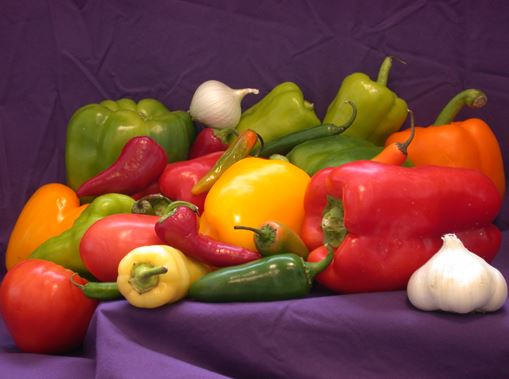
\includegraphics[height=0.6\textwidth,,keepaspectratio]{figures/2_2_1a}
  \caption{RGB Image}
  \label{fig:RGB Image Example}
\end{figure}

\vspace{40pt}
\begin{figure}[H]
  \centering
  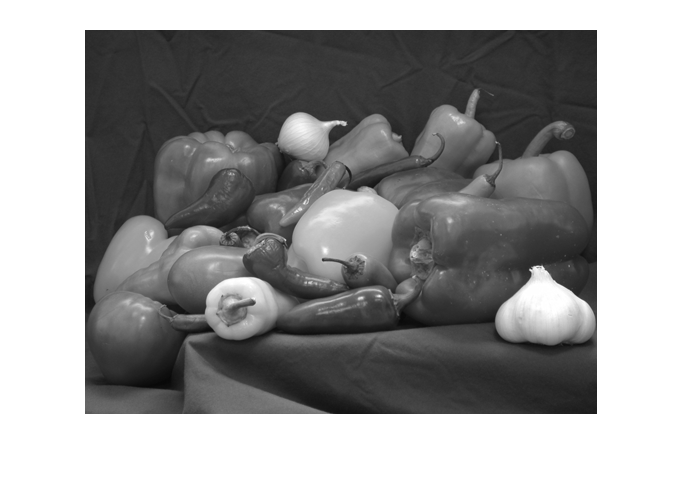
\includegraphics[width=0.9\textwidth]{figures/2_2_1b}
  \caption{Gray Scale Image}
  \label{fig:RGB to GrayScale Image}
\end{figure}

\subsection{Grayscale to Binary Image Conversion}
Binary images ~\cite{russ1995image} are the special kind of image whose intensity value has only two possible values. The image consists of two colors black and white and they are numerically represented by 0 and 1. The intensity value 0 means black and 1 means white. ``\Cref{fig:Grayscale to Binary Image Conversion} shows Grayscale to Binary Image conversion''.
\\

\begin{figure}[h]
  \centering
  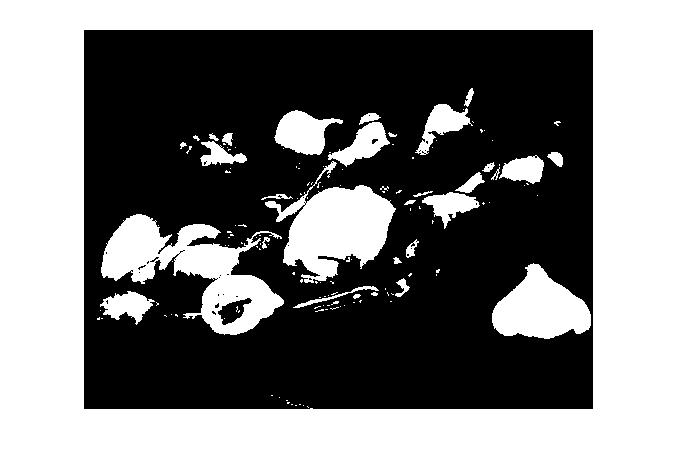
\includegraphics[width=0.9\textwidth]{figures/2_2_2}
  \caption{Grayscale to Binary Image Conversion}
  \label{fig:Grayscale to Binary Image Conversion}
\end{figure}

Basically, binary images are produced by thresholding a grayscale image or a  RGB  using a threshold intensity value and the objective of binarization is to separate the object from the background  image. Usually object color is white and referred to as the foreground color and the rest color is referred as the background color which is black. 

\section{Mask Image}

In image processing, a kernel, convolution matrix, or mask is a small matrix. It is used for blurring, sharpening, embossing, edge detection, image substraction, addition and more. This is accomplished by doing a convolution between a kernel and an image.  Masking involves setting some of the pixel values in an image to zero, or some other "background" value. A mask image is simply an image where some of the pixel intensity values are zero, and others are non-zero.


\subsection{Gaussian Filter}
Image blurring is achieved by convolving the image with a low-pass filter kernel. It is useful for removing noise. It
actually removes high frequency content (e.g: noise, edges) from the image resulting in edges being blurred when this
is filter is applied.

Probably the most useful filter (although not the fastest). Gaussian filtering is done by convolving each point in the input array with a Gaussian kernel and then summing them all to produce the output array. ``\Cref{fig:Gaussian} shows Gaussian Filtering''.

\begin{equation}
G(x,y) = \frac{1}{2 \pi \sigma ^{2}} e^{- \frac{x^{2} + y^{2}}{2 \sigma ^{2}}}
\label{2dgaussian}
\end{equation}

\vspace{50pt}
\begin{figure}[H]
  \centering
  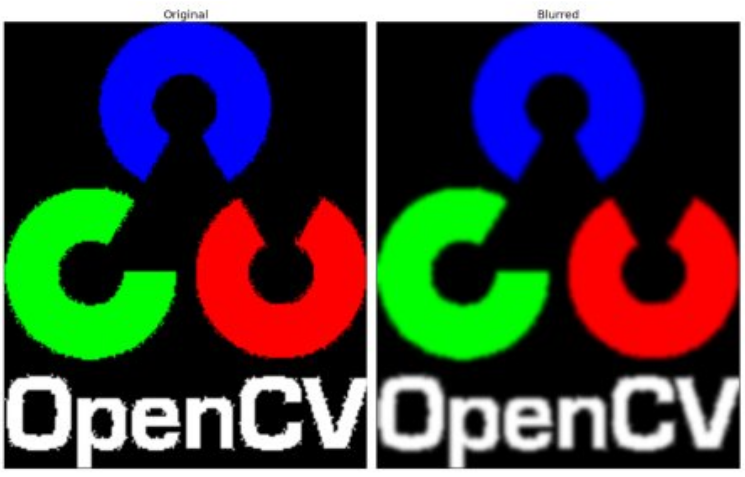
\includegraphics[width=0.9\textwidth]{figures/Gaussian}
  \caption{Gaussian Blur}
  \label{fig:Gaussian}
\end{figure}

\subsection{Median Filter}

The median filter run through each element of the signal (in this case the image) and replace each pixel with the median of its neighboring pixels (located in a square neighborhood around the evaluated pixel). ``\Cref{fig:Median} shows Median Filtering''.

\vspace{50pt}
\begin{figure}[H]
  \centering
  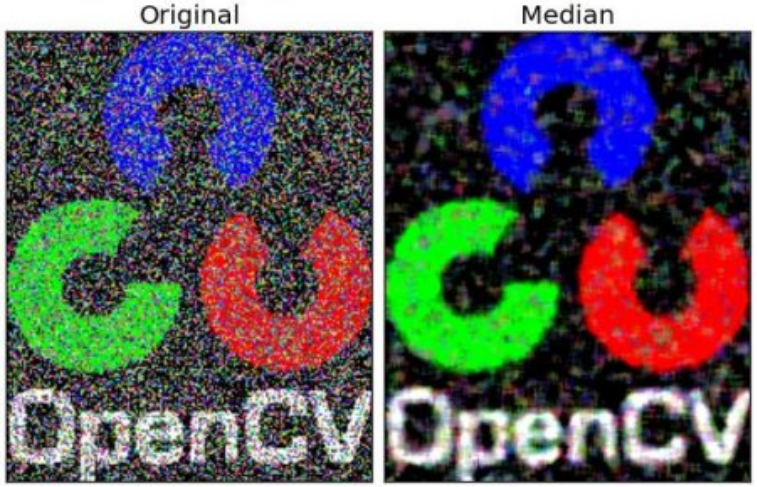
\includegraphics[height=0.4\textwidth,,keepaspectratio]{figures/Median}
  \caption{Median}
  \label{fig:Median}
\end{figure}

\section{Fundamental Operations in Morphological Image Processing}

Some of the more common operations of Morphological Image Processing are mentioned below:

\subsection{Erosion and Dilation}

The basic idea of erosion is just like soil erosion only, it erodes away the boundaries of foreground object (Always
try to keep foreground in white). So what does it do? The kernel slides through the image (as in 2D convolution). A
pixel in the original image (either 1 or 0) will be considered 1 only if all the pixels under the kernel is 1, otherwise it
is eroded (made to zero).

So what happens is that, all the pixels near boundary will be discarded depending upon the size of kernel. So the
thickness or size of the foreground object decreases or simply white region decreases in the image. It is useful for
removing small white noises (as we have seen in colorspace chapter), detach two connected objects etc.

Dilation is just the opposite of erosion. So it increases the white region in the image or size of foreground object increases. Normally, in cases like noise removal, erosion is followed by dilation. Because, erosion removes white noises, but it also shrinks our object. So we dilate it. Since noise is gone, they won’t come back, but our object area increases. It is also useful in joining broken parts of an object.

\begin{figure}[htp]

\centering

\includegraphics[width=.3\textwidth]{figures/Original}\hfill

\includegraphics[width=.3\textwidth]{figures/Erosion}\hfill

\includegraphics[width=.3\textwidth]{figures/Dilation}

\caption{From Left: Original Image, Eroded Image, Dilated Image}
\label{fig:Morpho}

\end{figure}


\subsection{Morphological Opening and Closing}
Opening is just another name of erosion followed by dilation. It is useful in removing noise, as explained above. ``\Cref{fig:Opening} shows Morphological Opening''.

Closing is reverse of Opening, Dilation followed by Erosion. It is useful in closing small holes inside the foreground
objects, or small black points on the object. ``\Cref{fig:Closing} shows Morphological Closing''.

\vspace{50pt}
\begin{figure}[H]
  \centering
  
\includegraphics[height=0.4\textwidth,,keepaspectratio]{figures/Opening}
  \caption{Morphological Opening}
  \label{fig:Opening}
\end{figure}

\vspace{50pt}
\begin{figure}[H]
  \centering
  
\includegraphics[height=0.4\textwidth,,keepaspectratio]{figures/Closing}
  \caption{Morphological Closing}
  \label{fig:Closing}
\end{figure}

\section{Image Segmentation}

In image processing, image segmentation is the process of partitioning a digital image into multiple segments (sets of pixels, also known as super-pixels). The goal of segmentation is to simplify and/or change the representation of an image into something that is more meaningful and easier to analyze.~\cite{shapiro2001computer} Image segmentation is typically used to locate objects and boundaries (lines, curves, etc.) in images. More precisely, image segmentation is the process of assigning a label to every pixel in an image such that pixels with the same label share certain characteristics. In our thesis we need image segmentation to segment out moving object. ``\Cref{fig:segmentation} shows an original image and segmented image''.

\begin{figure}[h]
  \centering
  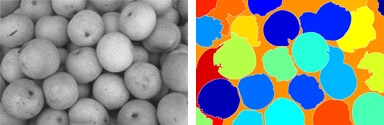
\includegraphics[width=0.8\textwidth]{figures/segmentation}
  \caption{Image Segmentation Example.}
  \label{fig:segmentation}
\end{figure}

\subsection{Region Growing}

Region growing is a simple region-based image segmentation method. It is also classified as a pixel-based image segmentation method since it involves the selection of initial seed points.

The main goal of segmentation is to partition an image into regions. Some segmentation methods such as thresholding achieve this goal by looking for the boundaries between regions based on discontinuities in grayscale or color properties. Region-based segmentation is a technique for determining the region directly. The basic formulation is:

\begin{enumerate}
\item Segmentation must be complete; that is, every pixel must be in a region.
\item Points in a region must be connected in some predefined sense.
\item Different regions must be disjoint.
\item All pixels in a common region must satisfy some common property.
\item If two regions are adjacent, they must be different in that predicate property.
\end{enumerate}

Seed points are selected to satisfy the requirements of the goal.

\section{Contour Detection}
Contours can be explained simply as a curve joining all the continuous points (along the boundary), having same color
or intensity. The contours are a useful tool for shape analysis and object detection and recognition.

Contours are the boundaries of a shape with same intensity. It stores the (x,y) coordinates of the boundary of a shape. But does it store all the coordinates ? That is specified by this contour approximation method. One such method, The Ramer–Douglas–Peucker algorithm, also known as the Douglas–Peucker algorithm and iterative end-point fit algorithm, takes a curve composed of line segments and finds a similar curve with fewer points.

``\Cref{fig:conapp} shows the Contour Approximation Procedure''.

\begin{figure}[h]
  \centering
  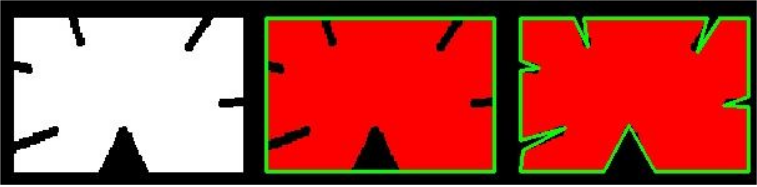
\includegraphics[width=0.8\textwidth]{figures/conapp.png}
  \caption{Contour Approximation}
  \label{fig:conapp}
\end{figure}

\section{Template Matching}
Template Matching is a method for searching and finding the location of a template image in a larger image. Simply slides the template image over the input image (as in 2D convolution) and compares the template and patch of input image under the template image.

\section{Conclusion}
We need these terminologies described above in our thesis. Image conversion transforms scanned colored image to greyscale. Smoothing eliminates unacceptable noise points in the scanned image. Morphological operations further clear out noise points and join adjacent broken curved segments. Contour detection detects majority of the plot contours and objects. Template matching segments out the numbered pixels and eliminates them from the original image. Region growing forms a connected whole Plot raster image.

\endinput



